\documentclass[11pt,a4paper]{article}

\usepackage[margin=2.2cm]{geometry}
\usepackage{amsmath,amssymb,amsthm}
\usepackage{booktabs}
\usepackage{array}
\usepackage{tabularx}
\usepackage[shortlabels]{enumitem}
\usepackage{xcolor}
\usepackage{tikz}
\usepackage{fancyhdr}
\usepackage{setspace}
\usepackage{microtype}
\usepackage{titlesec}
\usepackage{hyperref}
\usepackage[skins,breakable]{tcolorbox}

\usetikzlibrary{positioning,arrows.meta,calc,fit,shapes.geometric,matrix,decorations.pathreplacing}

\definecolor{ink}{HTML}{222222}
\definecolor{rulegray}{HTML}{444444}
\definecolor{boxline}{HTML}{666666}
\definecolor{boxfill}{HTML}{F4F4F4}
\definecolor{boxtitle}{HTML}{E8E8E8}
\definecolor{g1}{HTML}{D0D0D0}
\definecolor{g2}{HTML}{9A9A9A}
\definecolor{g3}{HTML}{5A5A5A}

\hypersetup{
  colorlinks=true,
  linkcolor=black,
  urlcolor=black,
  pdftitle={MTL 458 Lecture 15: Swapping Mechanism and Policy},
  pdfauthor={Minati De, IIT Delhi}
}

\setstretch{1.12}
\raggedbottom
\setlist[itemize]{leftmargin=1.3em,itemsep=0.28em,topsep=0.35em}
\setlist[enumerate]{leftmargin=1.5em,itemsep=0.35em,topsep=0.4em}

\titleformat{\section}
  {\Large\bfseries\color{ink}}{\thesection.}{0.6em}{}
  [{\color{rulegray}\titlerule[0.5pt]}]
\titleformat{\subsection}
  {\large\bfseries\color{ink}}{\thesubsection}{0.55em}{}
\titleformat{\subsubsection}
  {\normalsize\bfseries\color{ink}}{\thesubsubsection}{0.5em}{}

\titlespacing*{\section}{0pt}{1.35em}{0.7em}
\titlespacing*{\subsection}{0pt}{1.05em}{0.45em}

\pagestyle{fancy}
\fancyhf{}
\renewcommand{\headrulewidth}{0.4pt}
\renewcommand{\footrulewidth}{0.3pt}
\fancyhead[L]{\small\color{ink}MTL 458 \textbullet\ Operating Systems}
\fancyhead[R]{\small\color{ink}Lecture 15: Swapping Mechanism and Policy}
\fancyfoot[C]{\small\thepage}
\setlength{\headheight}{14pt}

% ---------------------------------------------------------------------------
% Boxes
% ---------------------------------------------------------------------------
\tcbset{
  commonbox/.style={
    colback=boxfill, colframe=boxline, boxrule=0.5pt,
    left=6pt, right=6pt, top=5pt, bottom=5pt,
    fonttitle=\bfseries, coltitle=black, colbacktitle=boxtitle,
    enhanced, sharp corners=south, breakable
  }
}
\newtcolorbox{keybox}[1][]{commonbox, title={#1}}
\newtcolorbox{quizbox}[1][]{commonbox, title={#1}}
\newtcolorbox{solbox}[1][]{commonbox, title={#1}}
\newtcolorbox{warnbox}[1][]{commonbox, title={#1}}
\newtcolorbox{defbox}[1][]{commonbox, title={#1}}

% Start a new page unless at least #1 of vertical space remains
\makeatletter
\newcommand{\keepspace}[1]{\par\penalty-100\begingroup
  \setlength{\dimen@}{#1}\dimen@ii\pagegoal\advance\dimen@ii-\pagetotal
  \ifdim\dimen@>\dimen@ii\ifdim\dimen@ii>\z@\vfil\fi\break\fi\endgroup}
\makeatother

\newcommand{\va}{\textit{VA}}
\newcommand{\pa}{\textit{PA}}
\newcommand{\vpn}{\textit{VPN}}
\newcommand{\pfn}{\textit{PFN}}
\newcommand{\ppn}{\textit{PPN}}
\newcommand{\pte}{\textit{PTE}}
\newcommand{\pde}{\textit{PDE}}

% Clock state: #1..#4 = use bits of frames 0..3, #5 = frame the hand points at
\newcommand{\clockstate}[5]{%
\begin{tikzpicture}[x=0.95cm,y=0.7cm,baseline=(current bounding box.center)]
  \foreach \i/\u in {0/#1,1/#2,2/#3,3/#4} {
    \pgfmathtruncatemacro{\shade}{\u==1 ? 30 : 8}
    \fill[black!\shade] (\i,0) rectangle (\i+1,1);
    \draw[black!60] (\i,0) rectangle (\i+1,1);
    \node[font=\small\bfseries] at (\i+0.5,0.5) {\i};
    \node[font=\scriptsize] at (\i+0.5,1.35) {use=\u};
  }
  \draw[black!60] (4,0) rectangle (4.8,1);
  \node[font=\small] at (4.4,0.5) {\ldots};
  \draw[-{Latex}, thick] (#5+0.5,-0.85) -- (#5+0.5,-0.08);
  \node[font=\scriptsize] at (#5+0.5,-1.15) {hand};
\end{tikzpicture}}

\begin{document}

% ===========================================================================
% Title
% ===========================================================================
\begin{center}
{\color{rulegray}\rule{\textwidth}{1.1pt}}\\[0.45em]
{\LARGE\bfseries Operating Systems}\\[0.25em]
{\Large\bfseries MTL 458 \textperiodcentered\ Lecture 15}\\[0.35em]
{\LARGE\bfseries Swapping: Mechanism and Policy}\\[0.35em]
{\large Minati De}\\[0.15em]
{\normalsize Department of Mathematics, Indian Institute of Technology Delhi}\\[0.35em]
{\color{rulegray}\rule{\textwidth}{1.1pt}}
\end{center}

\vspace{0.4em}
\begin{keybox}[What this lecture solves]
So far every page of every running process had to sit in physical
memory. Today we drop that assumption and let pages live on
\textbf{disk} until they are needed. Four questions drive the lecture:
\begin{itemize}
  \item How to run a process when there is \textbf{not enough physical
        memory}? \hfill \emph{(mechanism: page faults)}
  \item \textbf{When} should a page be moved from disk to memory?
        \hfill \emph{(policy: page selection)}
  \item \textbf{Which} page in memory should be replaced?
        \hfill \emph{(policy: page replacement)}
  \item How can the \textbf{LRU} page be approximated efficiently?
        \hfill \emph{(clock algorithm)}
\end{itemize}
\end{keybox}

\tableofcontents
\vspace{0.6em}
\noindent{\color{rulegray}\rule{\textwidth}{0.4pt}}

% ===========================================================================
\section{Motivation}
% ===========================================================================

\begin{keybox}[OS goal]
Support processes when there is \textbf{not enough physical memory}:
\begin{itemize}
  \item a \emph{single} process with a very large address space, or
  \item \emph{multiple} processes whose combined address spaces exceed
        physical memory.
\end{itemize}
User code should be \textbf{independent of the amount of physical
memory}. \textbf{Virtual memory}: the OS provides the illusion of more
physical memory than there really is.
\end{keybox}

\subsection{Walk-through: a program and its libraries}

The slides build up the following picture step by step.

\begin{enumerate}
  \item A \textbf{program} sits on disk. Its file contains \emph{code}
        and \emph{data}.
  \item When the OS runs it, it \textbf{creates} a \emph{virtual
        memory} (address space) for Process~1: code, data, heap at the
        bottom, stack at the top.
  \item \emph{What's in ``code''?} Not just the program's own code
        (\texttt{Prog}) but also \textbf{many large libraries}
        (\texttt{LibA}, \texttt{LibB}, \texttt{LibC}, \ldots), some of which are
        rarely or never used.
  \item \textbf{Question:} how do we avoid wasting \emph{physical} pages
        to back rarely used \emph{virtual} pages?
  \item Answer: only the pages actually needed so far are placed in
        physical memory --- e.g.\ \texttt{LibC} and \texttt{Prog}.
        \texttt{LibA} and \texttt{LibB} stay on disk.
  \item When the process \textbf{accesses LibB}, the OS
        \textbf{copies (or moves) it to RAM} and updates the mapping.
        This is called \textbf{paging in}.
\end{enumerate}

\begin{center}
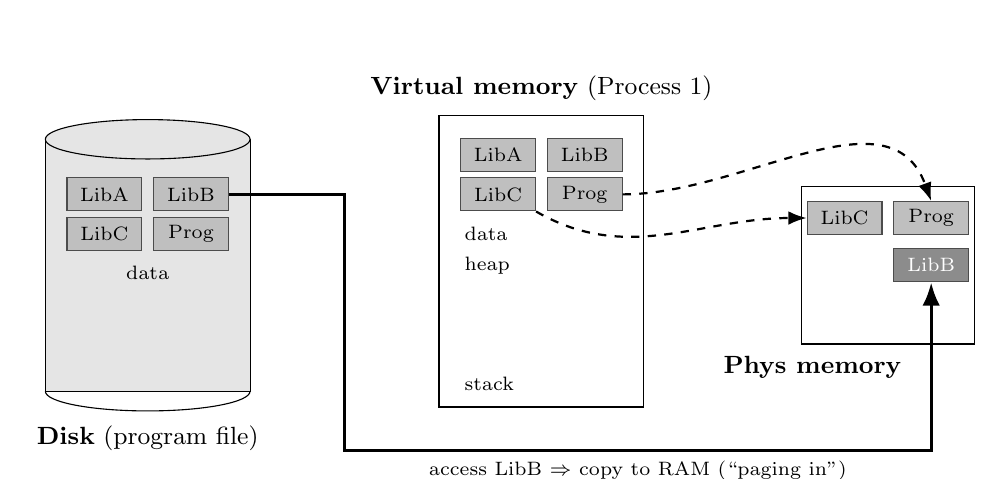
\begin{tikzpicture}[
  every node/.style={font=\small},
  pg/.style={draw=black!70, minimum width=0.95cm, minimum height=0.42cm,
             inner sep=1pt, font=\scriptsize},
  arr/.style={-{Latex}, thick}
]
  % disk
  \draw[fill=black!10] (0,0) rectangle (2.6,3.2);
  \draw[fill=black!10] (1.3,3.2) ellipse (1.3 and 0.25);
  \draw (0,0) arc (180:360:1.3 and 0.25);
  \node at (1.3,-0.6) {\textbf{Disk} (program file)};
  \node[pg, fill=black!25] (dA) at (0.75,2.5) {LibA};
  \node[pg, fill=black!25] (dB) at (1.85,2.5) {LibB};
  \node[pg, fill=black!25] (dC) at (0.75,2.0) {LibC};
  \node[pg, fill=black!25] (dP) at (1.85,2.0) {Prog};
  \node[font=\scriptsize] at (1.3,1.5) {data};

  % virtual memory
  \draw (5.0,-0.2) rectangle (7.6,3.5);
  \node at (6.3,3.85) {\textbf{Virtual memory} (Process 1)};
  \node[pg, fill=black!25] (vA) at (5.75,3.0) {LibA};
  \node[pg, fill=black!25] (vB) at (6.85,3.0) {LibB};
  \node[pg, fill=black!25] (vC) at (5.75,2.5) {LibC};
  \node[pg, fill=black!25] (vP) at (6.85,2.5) {Prog};
  \node[font=\scriptsize, anchor=west] at (5.2,2.0) {data};
  \node[font=\scriptsize, anchor=west] at (5.2,1.6) {heap};
  \node[font=\scriptsize, anchor=west] at (5.2,0.1) {stack};

  % physical memory
  \draw (9.6,0.6) rectangle (11.8,2.6);
  \node[anchor=east] at (11.0,0.3) {\textbf{Phys memory}};
  \node[pg, fill=black!25] (pC) at (10.15,2.2) {LibC};
  \node[pg, fill=black!25] (pP) at (11.25,2.2) {Prog};
  \node[pg, fill=black!45, text=white] (pB) at (11.25,1.6) {LibB};

  \draw[arr, dashed] (vC.south east) to[out=-30,in=180] (pC.west);
  \draw[arr, dashed] (vP.east) to[out=0,in=110] (pP.north);
  \draw[arr, very thick] (dB.east) -- (3.8,2.5) -- (3.8,-0.75)
        -- node[below, font=\scriptsize] {access LibB $\Rightarrow$ copy to RAM (``paging in'')}
        (11.25,-0.75) -- (pB.south);
\end{tikzpicture}\\[0.3em]
{\small Dashed: pages already resident. Solid: \texttt{LibB} paged in on its
first access. \texttt{LibA} is never touched, so it never uses a frame.}
\end{center}

The rest of the lecture explains \emph{why} this works (locality), the
\emph{mechanism} that makes it transparent (present bit + page fault),
and the \emph{policies} that decide what to bring in and what to throw out.

% ===========================================================================
\section{Why it works: locality and the memory hierarchy}
% ===========================================================================

\subsection{Locality of reference}

Leverage \textbf{locality of reference} within processes:
\begin{itemize}
  \item \textbf{Spatial locality:} a process tends to reference memory
        addresses \emph{near} previously referenced addresses
        (arrays, sequential code).
  \item \textbf{Temporal locality:} a process tends to reference memory
        addresses that it has \emph{referenced in the past}
        (loop variables, loop bodies).
  \item Processes spend the majority of their time in a small portion of
        their code. Estimate: \textbf{90\% of the time in 10\% of the code}.
\end{itemize}

\begin{keybox}[Implication]
\begin{itemize}
  \item A process only \emph{uses} a small amount of its address space at
        any moment.
  \item So only a small amount of the address space must be
        \textbf{resident in physical memory}. The rest can live on disk.
\end{itemize}
\end{keybox}

\subsection{Memory hierarchy}

Leverage the \textbf{memory hierarchy} of the machine architecture.
Each layer acts as a \textbf{``backing store''} for the layer above it.

\begin{center}
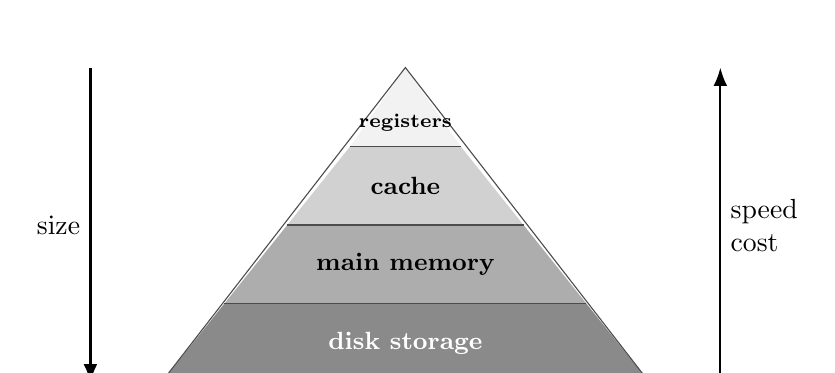
\begin{tikzpicture}[x=1cm,y=1cm]
  \fill[black!5]  (-0.7,3.0) -- (0.7,3.0) -- (0,4.0) -- cycle;
  \fill[black!18] (-1.5,2.0) -- (1.5,2.0) -- (0.7,3.0) -- (-0.7,3.0) -- cycle;
  \fill[black!32] (-2.3,1.0) -- (2.3,1.0) -- (1.5,2.0) -- (-1.5,2.0) -- cycle;
  \fill[black!46] (-3.1,0.0) -- (3.1,0.0) -- (2.3,1.0) -- (-2.3,1.0) -- cycle;
  \draw[black!70] (-3.1,0) -- (0,4.0) -- (3.1,0) -- cycle;
  \draw[black!70] (-0.7,3) -- (0.7,3);
  \draw[black!70] (-1.5,2) -- (1.5,2);
  \draw[black!70] (-2.3,1) -- (2.3,1);
  \node[font=\scriptsize\bfseries] at (0,3.3) {registers};
  \node[font=\small\bfseries] at (0,2.5) {cache};
  \node[font=\small\bfseries] at (0,1.5) {main memory};
  \node[font=\small\bfseries, white] at (0,0.5) {disk storage};
  \draw[-{Latex}, thick] (-4.0,4.0) -- (-4.0,0) node[midway, left] {size};
  \draw[-{Latex}, thick] (4.0,0) -- (4.0,4.0) node[midway, right, align=left] {speed\\cost};
\end{tikzpicture}
\end{center}

Going down: bigger, slower, cheaper per byte. Main memory acts as a
\emph{cache} for the disk, exactly as the hardware cache acts as a cache
for main memory.

% ===========================================================================
\section{Virtual memory intuition}
% ===========================================================================

\begin{defbox}[Idea]
The OS keeps \textbf{unreferenced pages on disk} --- a slower, cheaper
backing store than memory.
\end{defbox}

\begin{itemize}
  \item A process can run when \textbf{not all} of its pages are loaded
        into main memory.
  \item OS and hardware cooperate to provide the illusion of a
        \textbf{large disk as fast as main memory}:
        \begin{itemize}
          \item same \emph{behaviour} as if the whole address space were in
                main memory;
          \item hopefully similar \emph{performance}.
        \end{itemize}
\end{itemize}

\begin{keybox}[Requirements]
\begin{itemize}
  \item \textbf{Mechanism:} the OS must be able to identify the location
        of each page in the address space --- in memory or on disk.
  \item \textbf{Policy:} the OS must decide which pages live in memory and
        which on disk.
\end{itemize}
\end{keybox}

% ===========================================================================
\section{Mechanism: the present bit}
% ===========================================================================

Each page in the virtual address space maps to one of
\textbf{three locations}:

\begin{center}
\renewcommand{\arraystretch}{1.15}
\begin{tabular}{@{}lll@{}}
  \toprule
  \textbf{Location} & \textbf{Properties} & \textbf{PTE state} \\
  \midrule
  Physical main memory & small, fast, expensive & valid=1, present=1 \\
  Disk (backing store) & large, slow, cheap     & valid=1, present=0 \\
  Nothing (error)      & free                   & valid=0 \\
  \bottomrule
\end{tabular}
\end{center}

Extend page tables with an extra bit: \texttt{present}.
A \pte\ now holds: permissions (\texttt{r/w}), \texttt{valid}, \texttt{present}.
\begin{itemize}
  \item Page in memory: \texttt{present} bit \textbf{set} in the \pte;
        the \pte\ holds the \pfn.
  \item Page on disk: \texttt{present} bit \textbf{cleared}.
        \begin{itemize}
          \item The \pte\ points to the \textbf{block on disk}
                (the bits normally used for the \pfn\ hold the disk address).
          \item Referencing the page causes a \textbf{trap into the OS}.
          \item This trap is called a \textbf{page fault}.
        \end{itemize}
\end{itemize}

\begin{warnbox}[valid vs.\ present]
\textbf{valid=0}: the page is not part of the address space at all. Access
$\Rightarrow$ segmentation fault, process likely killed.\\
\textbf{valid=1, present=0}: the page is legal but currently on disk.
Access $\Rightarrow$ page fault, the OS fetches it, and the process
continues as if nothing happened.
\end{warnbox}

\subsection{Example: what if we access VPN \texorpdfstring{$0xb$}{0xb}?}

\begin{center}
\renewcommand{\arraystretch}{1.08}
\begin{tabular}{@{}c|cccc|cccc@{}}
  \toprule
  & \multicolumn{4}{c|}{\textbf{Before the access}} &
    \multicolumn{4}{c}{\textbf{After the page fault}} \\
  \textbf{VPN} & PFN & valid & prot & present & PFN & valid & prot & present \\
  \midrule
  0x0 & 10 & 1 & \texttt{r-x} & 1 & 10 & 1 & \texttt{r-x} & 1 \\
  0x1 & -- & 0 & --           & -- & -- & 0 & -- & -- \\
  0x2 & 23 & 1 & \texttt{rw-} & 0 & 23 & 1 & \texttt{rw-} & 0 \\
  0x3--0xa & -- & 0 & -- & -- & -- & 0 & -- & -- \\
  \textbf{0xb} & \textbf{28} & 1 & \texttt{rw-} & \textbf{0}
               & \textbf{16} & 1 & \texttt{rw-} & \textbf{1} \\
  0xc & 4  & 1 & \texttt{rw-} & 1 & 4  & 1 & \texttt{rw-} & 1 \\
  \bottomrule
\end{tabular}
\end{center}

\begin{itemize}
  \item VPN \texttt{0x0} and \texttt{0xc} are present: their PFN fields
        (10 and 4) are physical frames.
  \item VPN \texttt{0x2} and \texttt{0xb} are valid but \emph{not present}:
        their ``PFN'' fields (23 and 28) are really \textbf{disk block
        numbers}.
  \item Accessing VPN \texttt{0xb}: valid=1, present=0 $\Rightarrow$
        \textbf{page fault}. The OS reads disk block 28 into a free frame
        (frame 16), sets the \pte\ to \pfn=16, present=1, and retries.
\end{itemize}

% ===========================================================================
\section{Page-fault control flow}
% ===========================================================================

The \pte\ is used for data such as the \pfn\ of the page, \emph{or} for a
disk address. When the OS receives a page fault, it looks in the \pte\ and
issues the request to disk.

\begin{center}
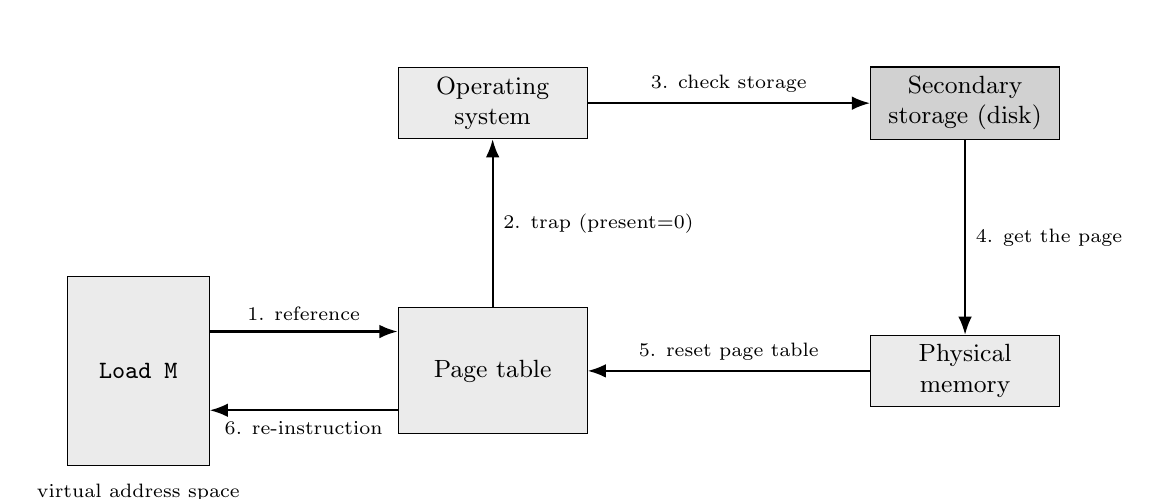
\begin{tikzpicture}[
  every node/.style={font=\small},
  box/.style={draw, fill=black!8, minimum width=2.4cm, minimum height=0.9cm, align=center},
  lab/.style={font=\scriptsize, fill=white, inner sep=1.5pt},
  arr/.style={-{Latex}, thick}
]
  \node[box, minimum height=2.4cm, minimum width=1.8cm] (va) at (0,0) {\texttt{Load M}};
  \node[below=0.1cm of va, font=\scriptsize] {virtual address space};
  \node[box, minimum height=1.6cm] (pt) at (4.5,0) {Page table};
  \node[box] (os) at (4.5,3.4) {Operating\\system};
  \node[box, fill=black!18] (disk) at (10.5,3.4) {Secondary\\storage (disk)};
  \node[box] (pm) at (10.5,0) {Physical\\memory};

  \draw[arr] ($(va.east)+(0,0.5)$) -- node[lab, above=2pt] {1. reference} ($(pt.west)+(0,0.5)$);
  \draw[arr] (pt.north) -- node[lab, right=2pt] {2. trap (present=0)} (os.south);
  \draw[arr] (os.east) -- node[lab, above=2pt] {3. check storage} (disk.west);
  \draw[arr] (disk.south) -- node[lab, right=2pt] {4. get the page} (pm.north);
  \draw[arr] (pm.west) -- node[lab, above=2pt] {5. reset page table} (pt.east);
  \draw[arr] ($(pt.west)+(0,-0.5)$) -- node[lab, below=2pt] {6. re-instruction} ($(va.east)+(0,-0.5)$);
\end{tikzpicture}
\end{center}

\begin{enumerate}
  \item \textbf{Reference:} the instruction \texttt{Load M} references a
        virtual address; the hardware looks up its \pte.
  \item \textbf{Trap:} the \pte\ has present=0, so the hardware raises a
        page fault and the OS takes over.
  \item \textbf{Check storage:} the OS reads the disk address from the \pte\
        and checks secondary storage for the page.
  \item \textbf{Get the page:} the page is read from disk into a free
        physical frame.
  \item \textbf{Reset page table:} the \pte\ gets the new \pfn\ and present=1.
  \item \textbf{Re-instruction:} the faulting instruction is restarted.
\end{enumerate}

\keepspace{8\baselineskip}
\subsection{Virtual memory mechanisms: the whole sequence}

Hardware and OS cooperate to translate addresses.
\begin{enumerate}
  \item First, hardware checks the \textbf{TLB} for the virtual address.
        If \emph{TLB hit}, address translation is done; the page is in
        physical memory.
  \item If \textbf{TLB miss}: hardware or OS walks the page tables. If the
        \pte\ says the page is present, the page is in physical memory
        (insert into TLB and retry).
  \item If \textbf{page fault} (present bit is cleared):
  \begin{itemize}
    \item Trap into the OS (page faults are \emph{not} handled by hardware,
          even on hardware-managed TLBs --- the disk I/O is too complex and
          slow, so the OS handles it).
    \item OS selects a \textbf{victim page} in memory to replace.
          Write the victim out to disk if it was modified
          (add \textbf{dirty bit} to the \pte).
    \item OS reads the referenced page from disk into memory.
    \item The page table is updated, the present bit is set.
    \item The process continues execution.
  \end{itemize}
\end{enumerate}

\begin{keybox}[What should the scheduler do?]
A page fault means a disk read, which takes \textbf{milliseconds}. The
faulting process is put in the \textbf{blocked} state while the I/O is in
flight, and the scheduler runs \textbf{another ready process}. When the
disk interrupt says the page has arrived, the faulting process becomes
ready again. This overlap of I/O and computation is exactly the
multiprogramming idea from the scheduling lectures.
\end{keybox}

% ===========================================================================
\section{Mechanism for continuing a process}
% ===========================================================================

Continuing a process after a page fault is \textbf{tricky}.
\begin{itemize}
  \item We want the page fault to be \textbf{transparent} to the user.
  \item A page fault may occur in the \textbf{middle of an instruction}:
        \begin{itemize}
          \item when the instruction itself is being fetched, or
          \item when data is being loaded or stored.
        \end{itemize}
  \item This requires \textbf{hardware support}:
        \textbf{precise interrupts} --- stop the CPU pipeline such that
        all instructions before the faulting instruction have completed,
        and those after it can be restarted (as if they never started).
\end{itemize}

\begin{keybox}[Complexity depends on the instruction set]
Can the faulting instruction be \textbf{restarted from the beginning}?
\begin{itemize}
  \item Example: \texttt{move +(SP), R2} --- an auto-increment
        addressing mode: it increments \texttt{SP} \emph{and} loads from
        memory.
  \item If the increment happens and then the load page-faults,
        simply re-running the instruction would increment \texttt{SP}
        \emph{twice}.
  \item So the hardware must \textbf{track side effects} so that they can
        be \textbf{undone} before restarting (or the instruction must be
        resumable from where it stopped).
\end{itemize}
\end{keybox}

% ===========================================================================
\section{Virtual memory policies}
% ===========================================================================

\begin{keybox}[Goal: minimize the number of page faults]
\begin{itemize}
  \item Page faults take \textbf{milliseconds} to handle (reading from disk).
  \item Implication: there is \textbf{plenty of time} for the OS to make a
        good decision (a few thousand instructions of policy code are
        nothing compared with one disk access).
\end{itemize}
\end{keybox}

\subsection{The two decisions}
The OS has two decisions:
\begin{itemize}
  \item \textbf{Page selection:} \emph{when} should a page (or pages) on
        disk be \textbf{brought into} memory?
  \item \textbf{Page replacement:} \emph{which} resident page (or pages) in
        memory should be \textbf{thrown out} to disk?
\end{itemize}

% ===========================================================================
\section{Page selection}
% ===========================================================================

When should a page be brought from disk into memory?

\subsection{Demand paging}
\begin{defbox}[Demand paging]
Load a page \textbf{only when a page fault occurs} on it.
\end{defbox}
\begin{itemize}
  \item Intuition: wait until the page \emph{absolutely must} be in memory.
  \item When the process starts, \textbf{no} pages are loaded in memory.
  \item Problem: pay the cost of a page fault for \textbf{every newly
        accessed page}.
\end{itemize}

\subsection{Prepaging (anticipatory, prefetching)}
\begin{defbox}[Prepaging]
Load a page \textbf{before} it is referenced.
\end{defbox}
\begin{itemize}
  \item The OS predicts future accesses (acts as an \emph{oracle}) and
        brings pages into memory early.
  \item Works well for some access patterns, e.g.\ \textbf{sequential}:
        if page \(P\) is brought in, page \(P+1\) is likely to be needed
        soon.
  \item \textbf{Problems:} prediction can be wrong.
        \begin{itemize}
          \item Wasted disk I/O for pages that are never used.
          \item The prefetched pages occupy frames, and may evict pages
                that \emph{were} going to be used, causing extra faults.
        \end{itemize}
\end{itemize}

\paragraph{Hints.} The conclusions slide also lists \textbf{hints}: the
application tells the OS about its future accesses, so the OS does not
have to guess.

\keepspace{10\baselineskip}
% ===========================================================================
\section{Page replacement}
% ===========================================================================

Which page in main memory should be selected as the \textbf{victim}?
\begin{itemize}
  \item Write the victim page out to disk if it is \textbf{modified}
        (\textbf{dirty bit} set).
  \item If the victim page is \textbf{not modified} (clean), just
        \textbf{discard} it --- the disk copy is still correct.
\end{itemize}

\begin{center}
\renewcommand{\arraystretch}{1.25}
\begin{tabularx}{\textwidth}{@{}>{\bfseries}l*{3}{>{\raggedright\arraybackslash}X}@{}}
  \toprule
  & \textbf{Rule} & \textbf{Advantages} & \textbf{Disadvantages} \\
  \midrule
  OPT  & Replace the page \textbf{not used for the longest time in the future}.
       & Guaranteed to minimize the number of page faults.
       & Requires the OS to predict the future. Not practical, but good for
         \textbf{comparison}. \\
  FIFO & Replace the page that has been \textbf{in memory the longest}.
       & Intuition: first referenced long time ago, done with it now.
         Fair: all pages receive equal residency. Easy to implement
         (circular buffer).
       & Some pages may \emph{always} be needed, yet FIFO still evicts them. \\
  LRU  & Least-recently-used: replace the page \textbf{not used for the
         longest time in the past}.
       & Intuition: use the past to predict the future. With locality,
         LRU approximates OPT.
       & Harder to implement: must track which pages have been accessed.
         Does not handle all workloads well. \\
  Random & Pick a random page.
       & Trivial to implement; avoids pathological corner cases.
       & Does not try to be intelligent; depends entirely on luck. \\
  \bottomrule
\end{tabularx}
\end{center}

\begin{keybox}[How to read the traces below]
Reference string \(0\,1\,2\,0\,1\,3\,0\,3\,1\,2\,1\); physical memory
(the ``cache'') holds \textbf{3 pages}.
\[
  \text{Hit rate} = \frac{\text{Hits}}{\text{Hits}+\text{Misses}}.
\]
The first three accesses are \textbf{compulsory (cold-start) misses}
under every policy: the cache starts empty.
\end{keybox}

\subsection{Tracing the optimal policy (OPT)}

\begin{center}
\renewcommand{\arraystretch}{1.08}
\begin{tabular}{@{}cccl@{}}
  \toprule
  \textbf{Access} & \textbf{Hit/Miss?} & \textbf{Evict} & \textbf{Resulting cache state} \\
  \midrule
  0 & Miss &   & 0 \\
  1 & Miss &   & 0, 1 \\
  2 & Miss &   & 0, 1, 2 \\
  0 & Hit  &   & 0, 1, 2 \\
  1 & Hit  &   & 0, 1, 2 \\
  3 & Miss & 2 & 0, 1, 3 \\
  0 & Hit  &   & 0, 1, 3 \\
  3 & Hit  &   & 0, 1, 3 \\
  1 & Hit  &   & 0, 1, 3 \\
  2 & Miss & 3 & 0, 1, 2 \\
  1 & Hit  &   & 0, 1, 2 \\
  \bottomrule
\end{tabular}
\end{center}

When 3 arrives, the cache is \(\{0,1,2\}\). Looking into the future
(\(0\,3\,1\,2\,1\)): 0 is needed next, then 1, and 2 is needed furthest
away $\Rightarrow$ evict \textbf{2}. When 2 arrives later, the future is
just \(1\); 0 and 3 are never used again, so either can go (the slide
evicts 3).
\[
  \text{Hit rate} = \frac{6}{6+5} = 54.6\%
\]
\emph{The future is not known} in real systems --- OPT is only a
yardstick.

\subsection{Tracing FIFO}

\begin{center}
\renewcommand{\arraystretch}{1.08}
\begin{tabular}{@{}cccl@{}}
  \toprule
  \textbf{Access} & \textbf{Hit/Miss?} & \textbf{Evict} & \textbf{Resulting cache state} \\
  \midrule
  0 & Miss &   & 0 \\
  1 & Miss &   & 0, 1 \\
  2 & Miss &   & 0, 1, 2 \\
  0 & Hit  &   & 0, 1, 2 \\
  1 & Hit  &   & 0, 1, 2 \\
  3 & Miss & 0 & 1, 2, 3 \\
  0 & Miss & 1 & 2, 3, 0 \\
  3 & Hit  &   & 2, 3, 0 \\
  1 & Miss & 2 & 3, 0, 1 \\
  2 & Miss & 3 & 0, 1, 2 \\
  1 & Hit  &   & 0, 1, 2 \\
  \bottomrule
\end{tabular}
\end{center}

The cache state is listed in arrival order: the leftmost page is the
``first in'', the next to be evicted.
\[
  \text{Hit rate} = \frac{4}{4+7} = 36.4\%.
\]
\begin{warnbox}[FIFO ignores importance]
Even though page 0 had been accessed a number of times, FIFO still
\textbf{kicks it out} (at the access to 3), because it arrived first.
\end{warnbox}

\keepspace{24\baselineskip}
\subsection{Another simple policy: Random}

Random picks a random page to replace under memory pressure. It doesn't
really try to be intelligent in picking which blocks to evict; its
performance depends entirely on how lucky \emph{Random} gets in its
choices. One possible run:

\begin{center}
\renewcommand{\arraystretch}{1.08}
\begin{tabular}{@{}cccl@{}}
  \toprule
  \textbf{Access} & \textbf{Hit/Miss?} & \textbf{Evict} & \textbf{Resulting cache state} \\
  \midrule
  0 & Miss &   & 0 \\
  1 & Miss &   & 0, 1 \\
  2 & Miss &   & 0, 1, 2 \\
  0 & Hit  &   & 0, 1, 2 \\
  1 & Hit  &   & 0, 1, 2 \\
  3 & Miss & 0 & 1, 2, 3 \\
  0 & Miss & 1 & 2, 3, 0 \\
  3 & Hit  &   & 2, 3, 0 \\
  1 & Miss & 3 & 2, 0, 1 \\
  2 & Hit  &   & 2, 0, 1 \\
  1 & Hit  &   & 2, 0, 1 \\
  \bottomrule
\end{tabular}
\end{center}

This run has 5 hits: \(5/11 = 45.5\%\). Over many runs, Random sometimes
matches OPT and sometimes does much worse.

% ===========================================================================
\section{Page replacement example: OPT vs.\ FIFO vs.\ LRU}
% ===========================================================================

\begin{quizbox}[Exercise from the slides]
Page reference string \texttt{A B C A B D A D B C B}, \textbf{three pages
of physical memory}. Fill in memory contents and count misses for OPT,
FIFO and LRU.
\end{quizbox}

\keepspace{22\baselineskip}
\begin{solbox}[Solution]
In each column the three entries are the frame contents \emph{after} the
access; \textbf{M} marks a miss, and (\(x\)) the evicted page.
\begin{center}
\renewcommand{\arraystretch}{1.08}
\setlength{\tabcolsep}{5pt}
\begin{tabular}{@{}c|ccc|ccc|ccc@{}}
  \toprule
  & \multicolumn{3}{c|}{\textbf{OPT}} & \multicolumn{3}{c|}{\textbf{FIFO}} & \multicolumn{3}{c}{\textbf{LRU}} \\
  \textbf{Ref} & frames & miss & evict & frames & miss & evict & frames & miss & evict \\
  \midrule
  A & A      & M &   & A     & M &   & A     & M & \\
  B & A B    & M &   & A B   & M &   & A B   & M & \\
  C & A B C  & M &   & A B C & M &   & A B C & M & \\
  A & A B C  &   &   & A B C &   &   & A B C &   & \\
  B & A B C  &   &   & A B C &   &   & A B C &   & \\
  D & A B D  & M & C & D B C & M & A & A B D & M & C \\
  A & A B D  &   &   & D A C & M & B & A B D &   & \\
  D & A B D  &   &   & D A C &   &   & A B D &   & \\
  B & A B D  &   &   & D A B & M & C & A B D &   & \\
  C & C B D  & M & A & C A B & M & D & C B D & M & A \\
  B & C B D  &   &   & C A B &   &   & C B D &   & \\
  \midrule
  \multicolumn{1}{c|}{\textbf{Misses}} & \multicolumn{3}{c|}{\textbf{5}} &
  \multicolumn{3}{c|}{\textbf{7}} & \multicolumn{3}{c}{\textbf{5}} \\
  \bottomrule
\end{tabular}
\end{center}
\begin{itemize}
  \item \textbf{OPT}, at D: future is \texttt{A D B C B}. C is used
        furthest away $\Rightarrow$ evict C. At C: future is \texttt{B}.
        A and D are never used again; evict either (here A).
  \item \textbf{FIFO}, at D: A came in first $\Rightarrow$ evict A ---
        right before A is needed again! This causes a chain of misses.
  \item \textbf{LRU}, at D: last uses are A@4, B@5, C@3 $\Rightarrow$
        evict C. At C: last uses are A@7, D@8, B@9 $\Rightarrow$ evict A.
\end{itemize}
Here LRU equals OPT (5 misses); FIFO is worst (7). The 3 initial misses
are compulsory for all.
\end{solbox}

% ===========================================================================
\section{What happens when we add more physical memory?}
% ===========================================================================

Intuitively, a bigger cache should never hurt. For FIFO this is
\textbf{false}.

\begin{quizbox}[FIFO performance may decrease!]
Access stream \texttt{A B C D A B E A B C D E}. Physical memory size 3
pages vs.\ 4 pages. How many misses with FIFO?
\end{quizbox}

\begin{solbox}[Answer: 3 pages $\to$ 9 misses, 4 pages $\to$ 10 misses]
\begin{center}
\renewcommand{\arraystretch}{1.05}
\setlength{\tabcolsep}{4pt}
\begin{tabular}{@{}c|cc|cc@{}}
  \toprule
  & \multicolumn{2}{c|}{\textbf{3 frames}} & \multicolumn{2}{c}{\textbf{4 frames}} \\
  \textbf{Ref} & queue (oldest first) & miss & queue (oldest first) & miss \\
  \midrule
  A & A       & M & A       & M \\
  B & A B     & M & A B     & M \\
  C & A B C   & M & A B C   & M \\
  D & B C D   & M & A B C D & M \\
  A & C D A   & M & A B C D &   \\
  B & D A B   & M & A B C D &   \\
  E & A B E   & M & B C D E & M \\
  A & A B E   &   & C D E A & M \\
  B & A B E   &   & D E A B & M \\
  C & B E C   & M & E A B C & M \\
  D & E C D   & M & A B C D & M \\
  E & E C D   &   & B C D E & M \\
  \midrule
  \multicolumn{1}{c|}{\textbf{Total}} & & \textbf{9} & & \textbf{10} \\
  \bottomrule
\end{tabular}
\end{center}
More memory, \emph{more} page faults. This is \textbf{Belady's anomaly}.
\end{solbox}

\subsection{Page replacement comparison}

Add more physical memory --- what happens to performance?
\begin{itemize}
  \item \textbf{LRU, OPT:} with more memory, \textbf{guaranteed} to have
        fewer (or the same number of) page faults.
        \begin{itemize}
          \item Smaller memory sizes are guaranteed to contain a
                \textbf{subset} of larger memory sizes.
          \item \textbf{Stack property:} the contents of a smaller cache
                are always a subset of the contents of a bigger cache
                (for the same reference string, at every point in time).
        \end{itemize}
  \item \textbf{FIFO:} with more memory, \emph{usually} fewer page faults.
        \begin{itemize}
          \item \textbf{Belady's anomaly:} may actually have \textbf{more}
                page faults!
        \end{itemize}
\end{itemize}

\begin{keybox}[Why the stack property rules out the anomaly]
For LRU, a cache of size \(k\) always holds the \(k\) most recently used
pages; a cache of size \(k+1\) holds the \(k+1\) most recently used ---
which includes those \(k\). So any hit with \(k\) frames is also a hit with
\(k+1\) frames. FIFO has no such property: in the trace above, after the
7th access the 3-frame cache holds \(\{A,B,E\}\) but the 4-frame cache
holds \(\{B,C,D,E\}\) --- not a superset.
\end{keybox}

% ===========================================================================
\section{Implementing LRU}
% ===========================================================================

\subsection{Software perfect LRU}
\begin{itemize}
  \item The OS maintains an \textbf{ordered list} of physical pages by
        reference time.
  \item When a page is referenced: move the page to the \textbf{front} of
        the list.
  \item When a victim is needed: pick the page at the \textbf{back} of the
        list.
  \item Trade-off: \textbf{slow on memory reference} (list update on every
        load/store!), fast on replacement.
\end{itemize}

\subsection{Hardware perfect LRU}
\begin{itemize}
  \item Associate a \textbf{timestamp register} with each page.
  \item When a page is referenced: store the system clock in its register.
  \item When a victim is needed: scan through the registers to find the
        oldest clock.
  \item Trade-off: \textbf{fast on memory reference}, slow on replacement
        (especially as the size of memory grows: a 4\,GB machine with 4\,KB
        pages has \(2^{20}\) pages to scan).
\end{itemize}

\begin{keybox}[In practice, do not implement perfect LRU]
\begin{itemize}
  \item LRU is an approximation (of OPT) anyway, so approximate more.
  \item Goal: find an \textbf{old} page, but not necessarily the very
        oldest.
\end{itemize}
\end{keybox}

% ===========================================================================
\section{Clock algorithm (approximating LRU)}
% ===========================================================================

\keepspace{18\baselineskip}
\begin{defbox}[Clock algorithm]
\textbf{Hardware:}
\begin{itemize}
  \item Keep a \textbf{use} (or \textbf{reference}) bit for each page frame.
  \item When a page is referenced: set its use bit to 1. (The hardware never
        clears it; only the OS does.)
\end{itemize}
\textbf{Operating system:}
\begin{itemize}
  \item Page replacement: look for a page with the use bit
        \textbf{cleared} (has not been referenced for a while).
  \item Implementation:
        \begin{itemize}
          \item Keep a pointer (the \textbf{clock hand}) to the last
                examined page frame.
          \item Traverse pages in a \textbf{circular buffer}.
          \item \textbf{Clear} use bits as you search.
          \item Stop when you find a page with an already cleared use bit;
                \textbf{replace this page}.
        \end{itemize}
\end{itemize}
\end{defbox}

\begin{verbatim}
while (true) {
    if (use[hand] == 1) {
        use[hand] = 0;              // give it a second chance
        hand = (hand + 1) % NFRAMES;
    } else {
        victim = hand;              // not recently used
        hand = (hand + 1) % NFRAMES;
        return victim;
    }
}
\end{verbatim}

A page with use=1 gets a ``second chance'': its bit is cleared, and it is
only evicted if it is still unused when the hand comes all the way back
round. If all bits are 1, the hand clears them all in one sweep and
evicts the frame it started at, so clock degenerates to FIFO.

\subsection{Clock: look for a page (slide animation)}

\begin{center}
\renewcommand{\arraystretch}{1.0}
\begin{tabular}{@{}c@{\hspace{1.5em}}l@{}}
\clockstate{1}{1}{0}{1}{0} &
  \parbox[c]{7.6cm}{\textbf{(1)} Need a victim. The hand is at frame 0:
  use=1.} \\[2.0em]
\clockstate{0}{1}{0}{1}{1} &
  \parbox[c]{7.6cm}{\textbf{(2)} Clear frame 0's bit, advance. Frame 1:
  use=1.} \\[2.0em]
\clockstate{0}{0}{0}{1}{2} &
  \parbox[c]{7.6cm}{\textbf{(3)} Clear frame 1's bit, advance. Frame 2:
  use=0 $\Rightarrow$ \textbf{evict page 2} because it has not been
  recently used. The new page is loaded into frame 2.} \\[2.0em]
\clockstate{1}{0}{0}{1}{3} &
  \parbox[c]{7.6cm}{\textbf{(4)} The hand has moved past the victim to
  frame 3. The process runs and \textbf{references page 0} again: hardware
  sets frame 0's use bit to 1. Later we need another victim; frame 3 has
  use=1.} \\[2.0em]
\clockstate{1}{0}{0}{0}{0} &
  \parbox[c]{7.6cm}{\textbf{(5)} Clear frame 3, wrap around to frame 0:
  use=1 (it was referenced in step 4).} \\[2.0em]
\clockstate{0}{0}{0}{0}{1} &
  \parbox[c]{7.6cm}{\textbf{(6)} Clear frame 0, advance. Frame 1: use=0
  $\Rightarrow$ \textbf{evict page 1} because it has not been recently
  used.}
\end{tabular}
\end{center}

(The slides draw frame 2's bit as 0 after the new page is loaded there; in
a real system the new page is accessed right away, so its bit would be 1.
Either way the second search starts at frame 3 and never reaches frame 2.)

Notice that page 0 survived both searches because it kept being used,
while pages 1 and 2 --- not touched since the last sweep --- were evicted.
That is the LRU-like behaviour, at the cost of one bit per frame.

\subsection{Considering dirty pages: (use bit, dirty bit) classes}

Evicting a dirty page costs a disk \emph{write} first; evicting a clean
page is free. So the enhanced clock considers \(\langle\text{ref bit},
\text{dirty bit}\rangle\) as an \textbf{ordered pair}:

\begin{center}
\renewcommand{\arraystretch}{1.18}
\begin{tabular}{@{}cl@{}}
  \toprule
  \textbf{(ref, dirty)} & \textbf{Meaning} \\
  \midrule
  \((0,0)\) & not recently used, clean --- \textbf{best page to replace} \\
  \((0,1)\) & not recently used, but modified (has to be written to disk first) \\
  \((1,0)\) & recently used, but clean (likely to be used again soon) \\
  \((1,1)\) & recently used and modified --- worst choice \\
  \bottomrule
\end{tabular}
\end{center}

The \textbf{first page in the lowest non-empty class} is selected as the
victim. (The classes are ordered so that ``recently used'' matters more
than ``dirty'': a recently used page will probably be needed again, which
would cost a whole fault.)

\subsection{Nth chance: not recently used}

Instead of one bit per page, keep an \textbf{integer}
\texttt{notInUseSince}: the number of sweeps since the page was last used.
Periodically sweep through all page frames:
\begin{verbatim}
if (page is used) {
    notInUseSince = 0;
} else if (notInUseSince < N) {
    notInUseSince++;
} else {
    reclaim page;
}
\end{verbatim}

\begin{itemize}
  \item ``Page is used'' means its hardware use bit is 1 (the OS clears it
        after reading it).
  \item A page is reclaimed only after it has been unused for \(N\)
        consecutive sweeps.
  \item Large \(N\): closer to true LRU (finer distinction between old and
        very old pages) but more sweeps to find a victim.
        Small \(N\): cheaper; \(N=0\) is the ordinary clock.
\end{itemize}

% ===========================================================================
\section{Summary}
% ===========================================================================

\begin{keybox}[Conclusions]
\begin{itemize}
  \item \textbf{Illusion of virtual memory:} processes can run when the
        sum of their virtual address spaces \(>\) the amount of physical
        memory.
  \item \textbf{Mechanism:}
        \begin{itemize}
          \item Extend the page table entry with a \textbf{present} bit.
          \item The OS handles page faults (page misses) by reading the
                desired page from disk.
          \item The hardware must support restartable instructions
                (precise interrupts).
        \end{itemize}
  \item \textbf{Policy:}
        \begin{itemize}
          \item Page selection --- demand paging, prefetching, hints.
          \item Page replacement --- OPT, FIFO, LRU, Random, others.
        \end{itemize}
  \item \textbf{Implementations} (clock) perform an
        \textbf{approximation of LRU}.
\end{itemize}
\end{keybox}

\begin{center}
\renewcommand{\arraystretch}{1.18}
\begin{tabular}{@{}lllll@{}}
  \toprule
  & \textbf{Uses} & \textbf{Stack property?} & \textbf{Cost} & \textbf{Notes} \\
  \midrule
  OPT    & future       & yes & impossible & lower bound on misses \\
  FIFO   & arrival time & no  & cheap      & Belady's anomaly \\
  Random & nothing      & no  & cheap      & depends on luck \\
  LRU    & past use     & yes & expensive  & approximates OPT \\
  Clock  & use bit      & ---  & cheap      & approximates LRU \\
  \bottomrule
\end{tabular}
\end{center}

\begin{warnbox}[Next lecture]
We now leave memory virtualization and move to the second ``easy
piece'': \textbf{concurrency} --- threads, shared data, and race conditions.
\end{warnbox}

\end{document}
